\documentclass[conference]{IEEEtran}
% RSS author kit. Use its bundled unmodified IEEEtran.cls V1.7a at final build.
\usepackage{times}
\usepackage[numbers]{natbib}
\usepackage{multicol}
\usepackage[bookmarks=true]{hyperref}
\hypersetup{hidelinks}
\usepackage{amsmath,amssymb,amsfonts}
\usepackage{graphicx}
\usepackage{booktabs}
\usepackage{tikz}
\usetikzlibrary{positioning,arrows.meta,calc,patterns}
\usepackage{pgfplots}
\pgfplotsset{compat=1.18}
\newcommand{\E}{\mathbb{E}}
\newcommand{\R}{\mathbb{R}}
\newcommand{\ind}{\mathbb{1}}
\pagestyle{empty}
\pdfinfo{
 /Author (Anonymous)
 /Title (What Transfers from Effect-Conditioned Action Pretraining to Vision-Language-Action Policies?)
 /Subject (RSS 2027 anonymous initial manuscript)
}
\begin{document}
\title{What Transfers from Effect-Conditioned Action\\Pretraining to Vision-Language-Action Policies?}
\author{Author Names Omitted for Anonymous Review}
\maketitle
\begin{abstract}
Numerical robot trajectories offer an opportunity to prepare a vision-language-action (VLA) policy before task-specific demonstrations are available. Yet an interaction carries several distinct supervisory signals: the actions taken, the motion requested by those actions, and the motion the robot actually executes. Which of these signals produces an initialization that remains useful for multimodal manipulation? We formulate two transfer contrasts among three intermediate pretraining regimes: a state-conditioned action prior ($P$), nominal-effect conditioning ($K$), and measured-effect conditioning ($D$). All regimes train the same SmolVLA action expert on matched trajectories using its native flow-matching objective; the temporary effect conditioner is removed before identical multimodal fine-tuning. In exploratory numerical-goal tests, $D$ attains 89.1\% and 78.1\% of 64 targets per seed, with substantially lower attainment when the supplied goal is masked or replaced. A separate low-demonstration task-training check achieves 158 successes in 200 rollouts. These observations motivate a paired Stage 2 study that will establish whether conditional action generation learned from nominal or measured effects transfers beyond an action prior and ordinary task training.
\end{abstract}
\IEEEpeerreviewmaketitle

\section{Introduction}
VLA policies learn manipulation from visual observations, language instructions and robot state \citep{black2025pi0,shukor2025smolvla,kim2024openvla}. Task-agnostic and action-expert pretraining show that robot experience can aid later task adaptation \citep{shi2026tap,hu2026arvla}. Yet a numerical trajectory contains distinct supervisory signals. \emph{Which should train the action generator before multimodal task learning?}

\begin{figure}[!b]
\centering
\resizebox{.97\columnwidth}{!}{% Audited sample means from 200 distinct start/chunk pairs; each replayed twice.
% These are scalar translation magnitudes, not reconstructed trajectories.
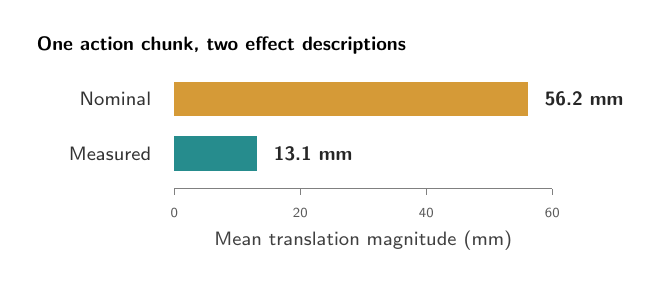
\begin{tikzpicture}[font=\sffamily\scriptsize]
\definecolor{nominalgold}{HTML}{D59A37}
\definecolor{measuredteal}{HTML}{268C8D}
\node[anchor=west,font=\sffamily\bfseries\scriptsize] at (0,2.15) {One action chunk, two effect descriptions};
\node[anchor=east,text=black!80] at (1.70,1.47) {Nominal};
\node[anchor=east,text=black!80] at (1.70,.78) {Measured};
\fill[nominalgold] (1.87,1.25) rectangle (6.365,1.69);
\fill[measuredteal] (1.87,.56) rectangle (2.922,1.00);
\node[anchor=west,font=\sffamily\bfseries\scriptsize,text=black!85] at (6.45,1.47) {56.2 mm};
\node[anchor=west,font=\sffamily\bfseries\scriptsize,text=black!85] at (3.01,.78) {13.1 mm};
\draw[black!50,thin] (1.87,.33) -- (6.67,.33);
\foreach \x/\lab in {1.87/0,3.47/20,5.07/40,6.67/60}{
  \draw[black!50,thin] (\x,.33) -- (\x,.25);
  \node[anchor=north,font=\sffamily\tiny,text=black!65] at (\x,.20) {\lab};
}
\node[anchor=north,font=\sffamily\scriptsize,text=black!75] at (4.27,-.08) {Mean translation magnitude (mm)};
\end{tikzpicture}

}
\caption{\textbf{Requested versus executed motion.} The same commands describe a nominal endpoint and produce a measured endpoint, motivating two distinct numerical conditioning signals (illustration).}
\label{fig:example}
\end{figure}

Figure~\ref{fig:example} illustrates the information difference. An action describes what the robot is asked to do, but need not specify what it actually accomplishes. For instance, a command requesting four centimeters of end-effector motion has a nominal displacement defined by the command convention and a measured displacement determined by the executed trajectory. The distinction is consequential because low-level control affects how requested actions are realized \citep{bronars2026tune}. In our exploratory robot-motion data, mean nominal translation was 56.2\,mm, compared with 13.1\,mm measured. Thus a single numerical interaction naturally provides \emph{three} possible training signals: the action itself, its nominal effect, and its observed effect.

These alternatives pose different learning problems. An \emph{action prior} learns how the robot tends to move from its current state. Conditioning on a \emph{nominal effect} asks the generator to turn a requested motion into actions. Conditioning on a \emph{measured effect} instead uses executed motion as the target specification. The scientific question is whether learning such conditional action generation improves subsequent manipulation, and whether observing actual effects adds value beyond command-derived goals. A comparison between a pretrained policy and standard fine-tuning cannot distinguish these possibilities.

We therefore isolate two downstream contrasts, nominal conditioning against an action prior and measured conditioning against nominal conditioning. For practical context, standard task fine-tuning ($S$) and compute-matched additional task fine-tuning ($E$) provide reference policies. Our hypothesis is that the native action expert can learn a reusable mapping from state and a compact motion specification to an action chunk. Although the temporary numerical conditioning token is discarded, the resulting action-generation parameters are retained and fine-tuned using task information conveyed by images and language. Figure~\ref{fig:transfer} illustrates this transition between conditioning interfaces.

The contribution is a controlled formulation of \emph{what transfers} from numerical robot experience, a native action-generation procedure that makes the supervisory alternatives comparable, and a hypothesis-driven evaluation that separates learning a numerical condition from transferring it to multimodal control. Initial evidence establishes goal-responsive action generation; the Stage 2 study resolves its downstream value.

\begin{figure*}[t]
\centering
\resizebox{.99\textwidth}{!}{% Fully editable scientific thesis figure. All paths correspond to the paper's transfer mechanism.
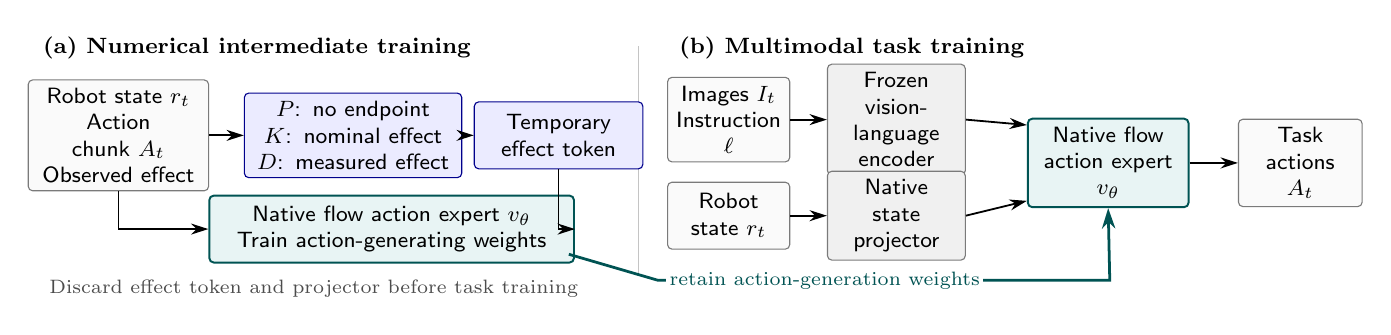
\begin{tikzpicture}[
  font=\sffamily\footnotesize, >=Stealth,
  input/.style={draw=black!52, fill=black!2, rounded corners=1.6pt, align=center,
     inner sep=3pt, minimum height=8.5mm},
  learned/.style={input, draw=blue!55!black, fill=blue!8},
  expert/.style={input, draw=teal!65!black, fill=teal!9, line width=.7pt},
  frozen/.style={input, fill=black!6},
  arr/.style={-{Stealth[length=2.2mm,width=1.4mm]},line width=.65pt},
  transfer/.style={-{Stealth[length=2.6mm,width=1.7mm]},line width=1.0pt,draw=teal!65!black}
]
% Section divider. Keep the logic explicit and the arrows non-crossing.
\node[anchor=west,font=\bfseries\footnotesize] at (0.12,3.08) {(a) Numerical intermediate training};
\node[anchor=west,font=\bfseries\footnotesize] at (8.20,3.08) {(b) Multimodal task training};
\draw[black!23] (7.80,.22) -- (7.80,3.10);
% Left: numerical trajectories, three interventions, same trained expert.
\node[input,text width=2.08cm] (data) at (1.20,1.97) {Robot state $r_t$\\Action chunk $A_t$\\Observed effect};
\node[learned,text width=2.55cm] (choice) at (4.18,1.97) {$P$: no endpoint\\$K$: nominal effect\\$D$: measured effect};
\node[learned,text width=1.93cm] (expertinput) at (6.79,1.97) {Temporary\\effect token};
\draw[arr] (data.east) -- (choice.west);
\draw[arr] (choice.east) -- (expertinput.west);
\node[expert,text width=4.42cm] (pre) at (4.67,.78) {Native flow action expert $v_\theta$\\Train action-generating weights};
\draw[arr] (expertinput.south) |- (pre.east);
\draw[arr] (data.south) |- (pre.west);
% Right: native modalities merged into same expert, no numerical-goal input at deployment.
\node[input,text width=1.34cm] (vl) at (8.95,2.17) {Images $I_t$\\Instruction $\ell$};
\node[frozen,text width=1.54cm] (encoder) at (11.08,2.17) {Frozen\\vision-language\\encoder};
\node[input,text width=1.34cm] (state) at (8.95,.95) {Robot\\state $r_t$};
\node[frozen,text width=1.54cm] (stateproj) at (11.08,.95) {Native\\state projector};
\node[expert,text width=1.83cm] (post) at (13.77,1.62) {Native flow\\action expert\\$v_\theta$};
\node[input,text width=1.36cm] (act) at (16.21,1.62) {Task actions\\$A_t$};
\draw[arr] (vl.east) -- (encoder.west);
\draw[arr] (state.east) -- (stateproj.west);
\draw[arr] (encoder.east) -- (post.155);
\draw[arr] (stateproj.east) -- (post.205);
\draw[arr] (post.east) -- (act.west);
% Transfer arrow under both halves; not connected to frozen backbone.
\draw[transfer] (6.92,.46) -- (8.05,.13) -- (13.79,.13) -- (post.south);
\node[font=\scriptsize,fill=white,inner sep=1.2pt,text=teal!65!black] at (10.17,.13) {retain action-generation weights};
\node[font=\scriptsize,text=black!70,anchor=west] at (.20,.02) {Discard effect token and projector before task training};
\end{tikzpicture}
}
\caption{\textbf{Shared action expert, different numerical supervision.} A robot observation $r_t$ and action chunk $A_t$ are shared by $P$, $K$ and $D$. A temporary effect token conditions the native action expert $v_\theta$ during numerical pretraining. The token is removed, while the trained action generator is retained for task conditioning from images $I_t$, instruction $\ell$ and robot state.}
\label{fig:transfer}
\end{figure*}

\section{Related Work}
\textbf{Pretraining robot action generators.} Prior work exploits unlabeled or task-agnostic robot experience in several forms. Manipulation-centric representation learning \citep{jiang2025mcr} and visual inverse dynamics on autonomous play in TAP \citep{shi2026tap} seek reusable experience before task adaptation. AR-VLA \citep{hu2026arvla} independently pretrains an autoregressive action expert, while APT \citep{xu2026apt} learns a vision-action prior before introducing language. Pose-VLA \citep{lin2026pose} instead emphasizes transferable pose representations. Together these approaches motivate staged learning, while leaving open how the \emph{choice of numerical supervision} affects transfer when the retained generator and trajectories are held fixed.

\textbf{Learning from anticipated and observed effects.} Predictive sensorimotor representation learning in PSR \citep{li2026psr} uses forecasts of future sensorimotor responses; SLIM \citep{wang2026slim} couples action reconstruction with future-latent prediction. Our comparison differs at the learning interface: a measured endpoint is supplied as a temporary \emph{condition} for generating actions, rather than predicted as a separate output. We use the flow-matching action expert of SmolVLA \citep{shukor2025smolvla,lipman2023flow,black2025pi0} and evaluate transfer on the language-conditioned LIBERO tasks \citep{liu2023libero}. This isolates the supervisory signal while keeping the deployed action-generation interface unchanged.

\section{Problem Formulation}
\subsection{Numerical interactions and endpoint effects}
Consider a corpus of robot observations and the action chunks executed between them. A training instance is $(r_t,A_t,r_{t+H})$, where $r_t\in\R^8$ contains end-effector pose and gripper coordinates and $A_t=(a_t,\ldots,a_{t+H-1})\in\R^{H\times7}$ contains $H=16$ Cartesian and gripper commands. Let $p_t\in\R^3$ and $R_t\in\mathrm{SO}(3)$ be the observed end-effector position and orientation. An \emph{endpoint effect} describes the net translation and rotation over a chunk; when given to the generator, it serves as a numerical motion goal. The \emph{measured effect} is
\begin{equation}
 e_t^{D}=\begin{bmatrix}p_{t+H}-p_t\\ \operatorname{Log}(R_t^\top R_{t+H})\end{bmatrix}\in\R^6,
 \label{eq:effect}
\end{equation}
Here $\operatorname{Log}:\mathrm{SO}(3)\to\R^3$ denotes the rotation-vector form of the matrix logarithm of the relative orientation. This measured effect is defined only after the chunk has been executed. In contrast, the \emph{nominal effect}, $e_t^{K}=G(r_t,A_t)$, is computed from the initial pose and the ideal command mapping, with its prescribed scaling, clipping, coordinate conventions and limits. It requires no subsequent observations or realized controller targets. The nominal map thus provides an outcome-free reference for the supervisory information contributed by measurement.

The three regimes are \emph{action prior} ($P$), which receives no informative effect; \emph{nominal-effect conditioning} ($K$), which receives $e_t^K$; and \emph{measured-effect conditioning} ($D$), which receives $e_t^D$. They share the same initial observations and action targets. In particular, $D$ replaces $K$'s condition rather than adding a measured residual, so the comparison evaluates two supervision procedures, not an isolated representation of hidden physical parameters.

\subsection{Transfer as a downstream quantity}
The question of transfer concerns manipulation after the numerical effect token has been removed. Let $I_t$ denote task images, $\ell$ an instruction, and $\pi_{m,b}$ the policy obtained from training regime $m\in\{P,K,D,S,E\}$ using $b$ demonstrations per task. Each policy uses the ordinary deployed inputs $(I_t,\ell,r_t)$. Let $Y_{m,b,j}\in\{0,1\}$ indicate success on task $j$, with expectation over the specified training and evaluation randomness. Across the fixed task set $\mathcal{T}$, define
\begin{equation}
 J_b(m)=\frac{1}{|\mathcal{T}|}\sum_{j\in\mathcal{T}}\E\!\left[Y_{m,b,j}\right],
 \label{eq:utility}
\end{equation}
where each task has equal weight. Our primary low-demonstration contrasts are
\begin{equation}
 C_1=J_{10}(K)-J_{10}(P),\qquad
 C_2=J_{10}(D)-J_{10}(K).
 \label{eq:contrasts}
\end{equation}
The first contrast, $C_1$, asks whether a nominal effect improves transfer beyond learning an action prior. The second, $C_2$, asks whether measured effects provide further downstream value relative to that nominal reference. Our directional hypotheses are $H_1:C_1>0$ and $H_2:C_2>0$, although both contrasts will be estimated in either direction. We prespecify five percentage points as the smallest gain of practical interest. Both hypotheses concern downstream task success, not endpoint attainment during pretraining.



\section{Intermediate Pretraining and Transfer}
The central methodological requirement is to vary \emph{supervision}, not the actions used for learning. Stage 2 therefore uses one fixed corpus of 250,000 numerical transitions from bounded arm and gripper interactions, with free-motion and contact attempts specified before collection. Neither task-success labels nor visual or linguistic inputs inform collection or intermediate training. Episodes are divided into disjoint splits before extracting action windows, and all numerical regimes use identical windows.
\subsection{Learning actions conditioned on effects}
Figure~\ref{fig:transfer} shows how the intervention is applied to a shared action expert. From one SmolVLA initialization, the vision-language backbone and robot-state projector remain frozen during intermediate learning. A temporary projector $h_{\eta}$ maps the numerical effect to a conditioning token, while the native action expert and its action-generation projections are trained. Because multiple action chunks can achieve the same endpoint, the native flow-matching objective learns conditional action generation without imposing a unique inverse or adding a dynamics-prediction head.

To make the conditions comparable, $z$ standardizes effects using only the nominal-effect statistics of the numerical training split. We set $q_t^P=0$, $q_t^K=z(e_t^K)$ and $q_t^D=z(e_t^D)$; hence $P$ has a neutral token, and $K$ and $D$ share one coordinate transformation. With Gaussian action noise $\epsilon$ and flow time $\tau\in[0,1]$, let $Z_\tau=(1-\tau)A_t+\tau\epsilon$ and $u_t=\epsilon-A_t$. Each regime $m\in\{P,K,D\}$ minimizes
\begin{equation}
 \mathcal{L}_m=\E_{t,\epsilon,\tau}\!\left[\left\|v_\theta\!\left(Z_\tau,\tau\mid r_t,h_{\eta}(q_t^m)\right)-u_t\right\|_2^2\right],
 \label{eq:fm}
\end{equation}
The loss is evaluated over the seven action coordinates. Projector initialization is matched to the native state-token scale, and a fixed 20\% of training windows mask effect-token attention. All regimes share training windows, optimization schedules and initial native parameters. Consequently, differences between their pretrained experts arise from the specified conditioning information.

\subsection{Transferring the action generator}
The temporary projector and effect token are removed before task learning. Only the updated native action-generation weights are retained, and the optimizer is reset. Every model is then fine-tuned with the same images, instructions, robot states and demonstrations; the vision-language backbone remains frozen, and the native robot-state projector is treated identically across conditions. The resulting policies have identical deployed inputs and architecture. Transfer is established only if learning to generate actions from numerical effects improves success when the expert is subsequently conditioned by multimodal task information.

\begin{table}[t]
\caption{\textbf{Numerical supervision and reference training regimes.} All downstream policies use the same deployed inputs and architecture.}
\label{tab:arms}
\centering
\footnotesize
\begin{tabular}{@{}p{.66cm}p{2.86cm}p{3.79cm}@{}}
\toprule
Arm & Numerical supervision & Training choice\\
\midrule
$P$ & Neutral effect token & Learn an action prior\\
$K$ & Nominal endpoint & Learn goal-conditioned actions from commands\\
$D$ & Measured endpoint & Learn goal-conditioned actions from observations\\
$S$ & None & Standard task fine-tuning\\
$E$ & None & Additional task training at matched extra compute\\
\bottomrule
\end{tabular}
\end{table}

Table~\ref{tab:arms} includes the practical reference conditions: $S$ starts task fine-tuning directly, whereas $E$ uses an equivalent additional compute allocation on the \emph{same} task demonstrations. These references test whether numerical pretraining is preferable to spending those resources on ordinary task learning.

\section{Preliminary Evidence}
The proposed transfer mechanism requires a distinguishable effect signal and an action expert capable of responding to numerical motion goals. We examine these prerequisites before asking whether their learned parameters improve a multimodal policy.

\textbf{Commanded and observed motion differ.} In 100 episodes from a fixed LIBERO-Goal scene (20,000 retained transitions), nominal motion averaged 56.2\,mm and 16.2$^\circ$, whereas measured motion averaged 13.1\,mm and 3.8$^\circ$. A linear predictor of the measured-versus-nominal discrepancy, using current robot state and actions, reduced held-out squared error by 99.0\% and 96.5\% relative to a training-mean predictor for translation and rotation. This pilot, which contained no movable-object contact, establishes that the command-derived and measured end-effector effects differ systematically under the selected controller.

\textbf{The action expert responds to numerical goals.} We trained each regime for 1,000 updates with two paired seeds, then evaluated 64 endpoint targets per seed from four held-out source episodes. At a joint tolerance of 10\,mm and 5$^\circ$, $D$ attained 89.1\% and 78.1\% of matched measured goals. Removing the conditioning reduced attainment to 12.5\% and 20.3\%; substituting an alternative goal reduced it to 6.3\% and 1.6\% (Fig.~\ref{fig:acquisition}a). This contrast demonstrates target-sensitive action generation beyond what is provided by the state-conditioned action prior.

\begin{figure*}[t]
\centering
% Audited exploratory acquisition results. Native measured-goal attainment for D;
% K on common measured goals is distribution shifted relative to its nominal training.
% X values are explicitly separated by seed for grayscale-safe grouped bars.
\begingroup
\pgfplotsset{every axis/.append style={
 font=\scriptsize,
 width=.455\textwidth,height=3.35cm,
 ymin=0,ymax=100,ytick={0,25,50,75,100},
 ylabel={Joint goal attainment (\%)},
 xmin=.45,xmax=3.55,
 xtick={1,2,3},
 axis y line*=left,axis x line*=bottom,
 ymajorgrids=true,grid style={draw=black!12},
 tick label style={font=\scriptsize},
 label style={font=\scriptsize},
 title style={font=\footnotesize\bfseries},
 bar width=9pt,
 mark=none,
 xtick style={draw=none},
}}
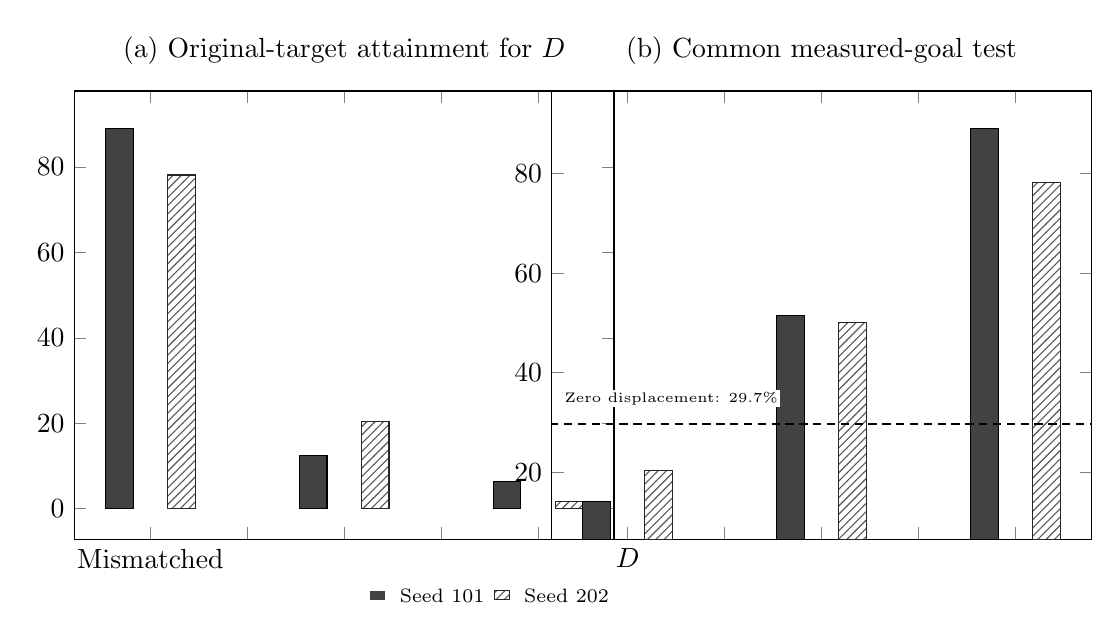
\begin{tikzpicture}
\begin{axis}[
 at={(0,0)},anchor=south west,
 xticklabels={Matched,Masked,Mismatched},
 title={(a) Original-target attainment for $D$}
]
\addplot+[ybar,mark=none,fill=black!74,draw=black,bar shift=0pt] coordinates {(.84,89.0625)(1.84,12.5)(2.84,6.25)};
\addplot+[ybar,mark=none,fill=white,pattern=north east lines,pattern color=black!65,draw=black!85,bar shift=0pt] coordinates {(1.16,78.125)(2.16,20.3125)(3.16,1.5625)};
\end{axis}
\begin{axis}[
 at={(.50\textwidth,0)},anchor=south west,
 xticklabels={$P$,$K$,$D$},
 title={(b) Common measured-goal test}
]
\addplot+[ybar,mark=none,fill=black!74,draw=black,bar shift=0pt] coordinates {(.84,14.0625)(1.84,51.5625)(2.84,89.0625)};
\addplot+[ybar,mark=none,fill=white,pattern=north east lines,pattern color=black!65,draw=black!85,bar shift=0pt] coordinates {(1.16,20.3125)(2.16,50.0)(3.16,78.125)};
\draw[densely dashed,thick] (axis cs:.60,29.6875) -- (axis cs:3.41,29.6875);
\node[fill=white,inner sep=.8pt,anchor=west,font=\tiny] at (axis cs:.66,34.8) {Zero displacement: 29.7\%};
\end{axis}
\begin{scope}[shift={(.31\textwidth,-.77cm)}]
  \fill[black!74] (0,0) rectangle (.19,.115);
  \node[anchor=west,font=\scriptsize] at (.25,.057) {Seed 101};
  \path[fill=white,pattern=north east lines,pattern color=black!65,draw=black!85] (1.58,0) rectangle (1.77,.115);
  \node[anchor=west,font=\scriptsize] at (1.83,.057) {Seed 202};
\end{scope}
\end{tikzpicture}
\endgroup

\caption{\textbf{Acquisition of numerical endpoint goals.} (a) Measured-effect conditioning under matched, masked and alternative goals. (b) Attainment on common measured goals for $P$, $K$ and $D$; $K$ was trained on nominal goals, so this is a shifted conditioning test. Bars denote the two seeds, with 64 targets each. The dashed line is the analytic zero-displacement reference, not an executed policy. Joint attainment requires 10\,mm and 5$^\circ$ accuracy. These tests establish acquisition, not multimodal transfer.}
\label{fig:acquisition}
\end{figure*}

Figure~\ref{fig:acquisition}b provides context on the common measured-goal set: attainment was 14.1\%/20.3\% for $P$, 51.6\%/50.0\% for $K$, and 89.1\%/78.1\% for $D$, against a 29.7\% analytic zero-displacement reference. The numerical comparison is not a downstream ranking: $K$ receives goals outside its nominal training distribution, and its strict in-domain nominal attainment was 1/64 and 0/64 despite improved continuous error under matched conditions. These complementary tests identify the acquired conditional behavior and motivate the downstream comparisons defined above.

\textbf{Multimodal task training is operational.} A separate standard policy ($S$), trained for 5,000 updates on ten demonstrations per task, succeeded in 158 of 200 exploratory LIBERO-Goal rollouts (79.0\%). This establishes an executable low-demonstration task setting in which the transfer hypotheses can be evaluated.

\section{Stage 2: Testing Transfer}
\subsection{Does numerical conditioning improve manipulation?}
The measured-effect acquisition results establish that a numerical motion goal can shape generated actions. The decisive question is whether the resulting action expert improves task success after its conditioning interface changes. We evaluate the same SmolVLA initialization on all ten LIBERO-Goal tasks, using 10 and 40 demonstrations per task with separate validation data. Each paired experiment keeps the numerical corpus, action windows, optimization schedule and deployment interface fixed across $P$, $K$ and $D$. Comparison with $S$ and $E$ then reveals whether the same resources are better used for intermediate numerical experience or additional task training.

For each regime we evaluate eight paired training seeds and 50 fixed resets per task. Numerical pretraining uses 5,000 updates, and task fine-tuning uses 10,000; a prespecified 5,000-update task checkpoint additionally tests whether any transfer benefit persists through training. To establish acquisition independently of task performance, native $K$ and $D$ goal response is evaluated with matched, masked and alternative goals. The acquisition criterion is a 10-percentage-point improvement in joint attainment over both masked conditioning and $P$, together with reduced translation and rotation error. These tests diagnose the proposed mechanism; they do not select the downstream policy or alter the fixed training schedule.

\subsection{When is a difference scientifically meaningful?}
Our primary estimates are the paired $C_1$ and $C_2$ differences at ten demonstrations per task. The independent unit is a training seed, with task outcomes averaged equally; resets are repeated measurements of a trained policy. We use two-sided 97.5\% paired confidence intervals to control the two primary comparisons, with the prespecified practical margin $\delta=0.05$. A meaningful gain requires the interval's lower bound to exceed $\delta$; a meaningful gain is excluded if the upper bound falls below $\delta$. An interval wholly within $[-\delta,\delta]$ supports practical equivalence, while other intervals remain inconclusive. These conclusions depend on the estimated paired variability rather than episode counts alone.

\begin{table}[t]
\caption{\textbf{Interpretation of the primary transfer contrasts.} The table specifies conclusions sought in Stage 2, not results already observed.}
\label{tab:outcomes}
\centering
\footnotesize
\begin{tabular}{@{}p{2.38cm}p{5.09cm}@{}}
\toprule
Supported outcome & Training implication\\
\midrule
$C_1$ gain; $C_2$ equivalent & Nominal conditioning helps beyond an action prior; measured labels confer no resolved practical benefit.\\
Meaningful $C_2$ gain & Measured labels outperform the ideal command map; test practical value against $S/E$.\\
Negative $C_2$ & Nominal conditioning is preferable if competitive with $S/E$.\\
$S$ or $E$ performs best & Prefer standard or extra task training.\\
Acquisition not established & Compare procedures, without attributing differences to learned goal conditioning.\\
Unresolved intervals & No supervision preference is established.\\
\bottomrule
\end{tabular}
\end{table}

Table~\ref{tab:outcomes} makes the planned inferences explicit. Attribution to \emph{transfer of goal conditioning} requires evidence that the corresponding numerical objective was acquired. If acquisition is not established, any task difference remains a comparison between training procedures rather than an identified goal-conditioning mechanism. Early and final task checkpoints distinguish temporary improvement from a persistent advantage without choosing a favorable checkpoint.

\subsection{Distinguishing supervision from controller calibration}
The measured-versus-ideal discrepancy observed in the pilot was largely predictable from robot state and commands. On the full corpus we will separately characterize residual predictability for free-motion and observed contact transitions, where such contacts occur. Accordingly, $C_2$ compares measured outcomes with an \emph{ideal command map}, not with a learned calibrated controller. A positive result would motivate a calibrated-nominal diagnostic, while a precise negligible difference would support the adequacy of nominal supervision within the evaluated regime. The negotiated Extension Charter may include this calibration test or an intermediate-training dose comparison as explanatory diagnostics while retaining the primary five-regime study.

\section{Conclusion}
Actions, requested motion, and measured motion pose distinct learning problems for a shared action generator. Our matched formulation and pilot establish goal-responsive numerical pretraining without changing the deployed VLA. Stage 2 will test whether the resulting initialization improves multimodal manipulation and which supervision is worth collecting.

\clearpage
\bibliographystyle{plainnat}
\bibliography{references}
\end{document}